\FloatBarrier
\section{Setup Details}
\label{app:setup}

\begin{table}[htbp]
\centering
\small
\setlength{\tabcolsep}{3pt}
\begin{tabular}{p{0.3\columnwidth}p{0.64\columnwidth}}
\toprule
Proposals & 1,200 requests per round (40 topic prompts $\times$ 30), $T{=}1.0$, top-$p$ 0.95, $\le$300 tokens; kept if $\ge$40 characters, with a digit and a question mark, and not a duplicate \\
Planted problems & 200 premise-deleted and 200 intact GSM-Symbolic variants per round, disjoint from the evaluation probe \\
Admission & $G{=}8$ samples, $T{=}1.0$, $\le$1,024 tokens; $p$ = share of the most frequent parsed answer (unparsed samples count in the denominator); admit if $0.25 \le p \le 0.75$ \\
Training & 60 steps per round, 32 problems $\times$ 8 rollouts; reward 1 for matching the group majority; advantage = reward $-$ group mean, not divided by the group's standard deviation; one on-policy update per batch, so no ratio clipping is needed; no KL term; learning rate $10^{-6}$ (constant); gradient clip 1.0; full-parameter, bf16 weights with fp32 master \\
Optimiser & 8-bit AdamW on GPU (Qwen3-4B, Phi-4-mini, Llama-3.2-3B); fp32 AdamW on CPU (Qwen3-8B, Qwen3-14B) \\
Labels & 200 admitted proposals per round, 8 judges $\times$ 25 (10 $\times$ 20 for the first four round-1 samples) \\
UMWP probe & 600 unanswerable + 600 answerable originals, 8 samples, $T{=}1.0$ \\
Accuracy & greedy; MATH-500, 1,000 further MATH test problems, 500 GSM8K test problems \\
Compute & 8 NVIDIA RTX PRO 5000 (72\,GB) per host, 3 hosts; about 1\,h (4B) to 3\,h (14B) of training per round; about 1,400 GPU-hours in total (1,300--1,600), 435 of them for the R-Zero replication \\
Software & vLLM 0.11.0 \citep{kwon2023vllm} for sampling, PyTorch 2.8.0, transformers 4.57.1, bitsandbytes 0.48.1 8-bit AdamW, our own policy-gradient trainer; no hyper-parameter search \\
\bottomrule
\end{tabular}
\caption{Loop settings. Base models see the problem followed by ``Let's think step by step and output the final answer within \textbackslash boxed\{\}''; instruction-tuned models see the same text in their chat template. The supplementary material lists the 40 topic prompts and the proposer's instruction template.}
\label{tab:hparams}
\end{table}

\paragraph{Answer parsing in the loop (filter reading).} Generation by a base model stops at a new ``Question:'' or ``Problem:'' line. We take the last boxed expression; otherwise an explicit ``Answer: unknown'' counts as abstention; otherwise the text after ``\#\#\#\#''; otherwise the last number. Numbers are normalised before comparison. Behavioural numbers use the strict reading of \S\ref{sec:setting} instead (Appendix~\ref{app:readings}).

\paragraph{Planted problems.} Admitted premise-deleted problems make up 11.5--22.8\% of the training sets of the full curricula (Qwen3-4B, Qwen3-8B and Phi-4-mini; 45 runs) and admitted intact ones 6.3--17.7\%; from round two on, every run admits more deleted than intact ones. None of the 23,241 judge labels concerns a planted problem.

\paragraph{Training-set size and passes.} Every round trains for 60 steps of 32 problems, drawn by cycling through a reshuffled training set, so a set of $n$ problems is passed over $1{,}920/n$ times, with eight rollouts per pass. The admitted set shrinks as the curriculum drifts, and the number of passes grows (Figure~\ref{fig:sizes} in Appendix~\ref{app:results}).

\paragraph{Controls and variants.} The \emph{solvable-only} curriculum trains on the admitted proposals that the judges, labelling every admitted proposal, call solvable, plus the admitted intact planted problems, and no deleted ones. The \emph{size-matched random loop} admits, in every round, a random subset of the band of the size the abstention guard admits (62--69\% of the full curriculum at round three). The \emph{same-size contrast} trains one round from the round-2 solver either on the solvable proposals of the round-3 admitted set plus its intact planted problems, or on a random subset of that set of the same size (148--177 problems, of which 20--39 are premise-deleted). The \emph{same-size contrast without planted problems}, registered before any of its new runs existed, replaces in place each premise-deleted problem of that random subset (20--39 per seed) with a random admitted proposal not already in it, leaving the size, the order of the other problems and every setting unchanged; its runs were trained three days after the others, and GPU sampling is not bitwise reproducible. Of its problems, 103--117 are ill-posed proposals (79--95 in the random subset) and 14--26 intact planted problems, against none and 60--82 in the solvable set. Putting the planted premise-deleted problems back in place of these proposals changes the rate by +0.3 points on average (95\% CI $[-3.0, 3.6]$; higher in three of five seeds; answers read as in \S\ref{sec:setting}); this and the difference without them add up to the same-size contrast by construction. With the abstention option, one round on the solvable problems, on the random subset and on the subset without planted problems abstains on 70, 71 and 68\% of the unanswerable UMWP questions and on 2, 2 and 2\% of the answerable ones (seed means, five seeds). The Absolute-Zero-style band admits $0 < p < 1$. The co-evolving proposer is fine-tuned after each round for two epochs on the proposals the band admitted (learning rate $10^{-5}$).

\FloatBarrier
\section{Judges and Their Validation}
\label{app:judge}

\paragraph{Judges.} Each judge is a Claude Opus agent (Opus 5 series, September 2026; the blind re-judging and the R-Zero labels used \texttt{claude-opus-5-5}) with a fresh context and shell access, which fetches its batch of problems with one command and may check computations locally. It receives the following definitions (verbatim): ``These were written by a [model] language model and ADMITTED by a self-play filter. For EACH question decide: SOLVABLE -- the text determines a unique numeric answer (state it briefly in the note); UNSOLVABLE -- a needed quantity/relation is missing, or the text is self-contradictory, so no unique answer exists; AMBIGUOUS -- two reasonable readings give different answers. Be strict: a default assumption you would have to invent makes it UNSOLVABLE. Confidence 0-1, note $\le$ 20 words.'' The framing sentence is the same in every round.

\paragraph{Validation.} Figure~\ref{fig:validation} collects the checks. On UMWP, the 200 unanswerable questions were stratified by source and category and the 200 answerable ones by source. On 200 planted problems of known status, the judge labels 92 of 100 deletions and 12 of 100 intact problems ill-posed; the notes of all eight deletions judged solvable give an answer that differs from the original's, i.e.\ these deletions left the problem solvable. An LLM reader compared the 12 intact problems with their reference answers and with the judge's labels for other instances of the same template$^{\dagger}$: 7 are genuine defects of the instance (one needs 112\% of a working day, two assume four weeks in April or July, and four are ambiguous, three of them from one template whose premise sentence, placed after the question, reads as a final total), and 5 are judge false positives, four of which contradict the judge's solvable label for another instance of the same template. The false-positive rate on well-posed intact problems is thus about 5\% (5 of 93). Re-judging two samples with new judges and reversed order reproduces the ill-posed share within 2.5 points; disagreements concentrate on the boundary between unsolvable and ambiguous, which is why we report their sum.

\begin{figure}[htbp]
\centering
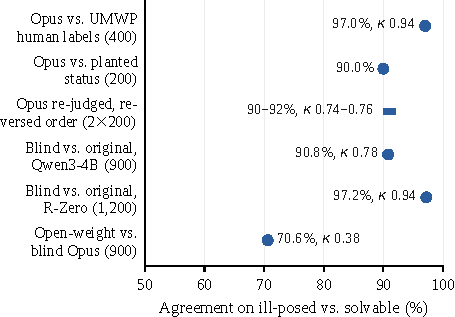
\includegraphics[width=\columnwidth]{figures/figA_validation.pdf}
\caption{Agreement on ill-posed vs.\ solvable across judges and against human labels, with Cohen's $\kappa$ (number of problems in parentheses).}
\label{fig:validation}
\end{figure}

\paragraph{Human annotation.} We sampled 240 of the 900 problems re-judged blind (Qwen3-4B, seeds 0--2, rounds 1, 3 and 5; 80 per round, 26--27 per seed and round), shuffled them under neutral identifiers and gave them to two external annotators, PhD students in mathematics (fourth and third year), with the instruction: ``Label each question with exactly one of: S (SOLVABLE): the text determines a unique answer without inventing any assumption. U (UNSOLVABLE): a needed quantity or relation is missing, or the text is self-contradictory, so no unique answer exists. A (AMBIGUOUS): two reasonable readings give different answers. Be strict: if you would have to invent a default assumption to get a number, label U.'' They worked independently, without LLM assistance and without having read this paper or seen model outputs; a postdoctoral mathematician adjudicated the 17 disagreements, seeing only the two labels, not the round or any judge label. Each was paid USD 500 for about five hours. The analysis plan and script were registered after the annotation but before the labels were joined with the round and judge information (Appendix~\ref{app:prereg}, deviation 14). Figure~\ref{fig:human} shows the results; on the same problems, blind Opus agrees with the annotators at $\kappa{=}0.89$ and measures a somewhat larger drift on the same problems ($+26.2$; paired difference $+6.2$, CI $[0.0, 12.5]$). The confidence intervals come from an item bootstrap within the three runs. The estimated rise is positive in every seed ($+14.8$, $+22.2$ and $+23.1$ points; with 26--27 problems per cell, each per-seed interval reaches 0) and under each annotator's labels alone ($+18.8$ and $+17.5$, both intervals above 0); a logistic trend over rounds gives an odds ratio of 1.28 per round (95\% CI $[1.07, 1.52]$). Corrected for the judge's per-round error rates estimated from these 240 problems, the blind Opus drift on all 900 problems is $+17.2$ (Rogan--Gladen, CI $[2.8, 28.1]$) or $+18.4$ points (two-phase estimator, CI $[9.1, 27.3]$)$^{\dagger}$, against $+24.7$ uncorrected.

\begin{figure}[htbp]
\centering
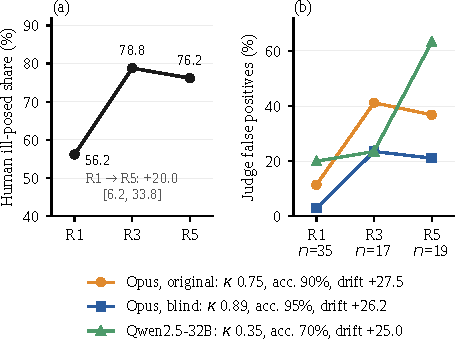
\includegraphics[width=\columnwidth]{figures/figA_human.pdf}
\caption{Human annotation of 240 Qwen3-4B problems. (a)~Ill-posed share under the final human labels, with the change from round one to five and its 95\% CI. (b)~False-positive rate of each judge: the share of human-solvable problems ($n$ per round) that it calls ill-posed; legend: binary $\kappa$ and accuracy against the final human label, and the drift the judge measures on the same 240 problems. The annotators agree at $\kappa{=}0.87$ (three classes, CI $[0.81, 0.92]$) and $0.91$ (ill-posed vs.\ solvable, $[0.85, 0.96]$).}
\label{fig:human}
\end{figure}

\paragraph{Blind re-judging.} We re-judged blind the labelled samples of Qwen3-4B (seeds 0--2, rounds 1, 3 and 5) and of R-Zero. We shuffled the problems under neutral keys into one file whose name carried no information about their origin; each judge fetched only its own lines, and we checked afterwards which files each judge had read. In the R-Zero re-judging (49 judge batches), one batch of 25 was discarded and re-judged, as the pre-registered protocol required, because its judge had read the output of its own background computation, which the check did not permit.

\FloatBarrier
\section{Pre-Registration and Outcomes}
\label{app:prereg}

\paragraph{Procedure.} We pre-registered eleven sets of predictions. For each, we wrote the predictions, thresholds, analysis scripts and the conditions for stopping a run before generating the data, and appended their SHA-256 hashes, with timestamps, to an append-only log that we maintain ourselves; from the third set on, most analysis scripts were reviewed by LLM agents before their first run. Figure~\ref{fig:prereg} summarises the outcomes, Table~\ref{tab:claims} maps each claim of the abstract to its evidence and registration status, and the supplementary material lists all 136 predictions (S1--S136) with their thresholds and outcomes. Its software and data archives also contain the registration log with the registered documents and scripts of every study reported here and a script that recomputes their hashes, all prompts (including the corrected abstention prompt), the item identifiers, seeds and analysis scripts, label tables that give the source of every label, and our patch to the R-Zero code.

\begin{figure}[htbp]
\centering
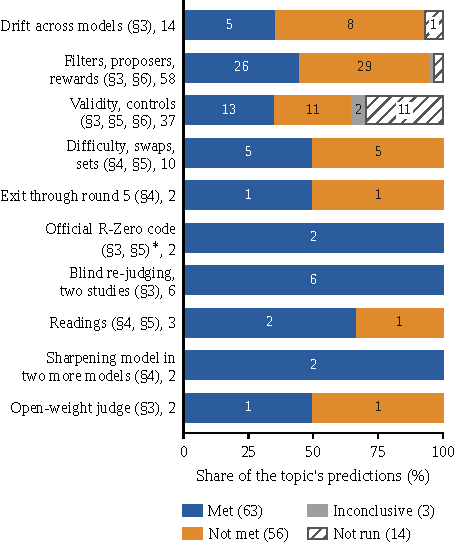
\includegraphics[width=\columnwidth]{figures/figA_prereg.pdf}
\caption{Outcomes of the pre-registered predictions by topic (number of predictions after each topic; counts in the bars). Met / not met: the outcome meets or misses the pre-registered criterion. The two unlabelled segments of filters, proposers and rewards are 1 inconclusive and 2 not run. $^{\ast}$Both R-Zero predictions are met by the pre-registered analysis script, which we ran once all computation had ended, before the times fixed for it; the runs at those times give byte-identical output (deviation 9).}
\label{fig:prereg}
\end{figure}

\begin{table*}[tp]
\centering
\small
\setlength{\tabcolsep}{4pt}
\begin{tabular}{p{0.34\textwidth}p{0.14\textwidth}p{0.46\textwidth}}
\toprule
Claim of the abstract & Evidence & Registration and outcome \\
\midrule
The ill-posed share of admitted problems rises by 11.5--27 points within two rounds & \S3, Table~\ref{tab:drift} & Unsolvable share: S3 (Qwen3-4B/8B) and S26 (Phi-4-mini) met; S38 (Qwen3-14B, $+6.0$ against $+10$) not met; Llama-3.2-3B drift (S2, S4) not met. The ill-posed share is reported alongside \\
\ldots also under blind re-judging, an open-weight judge and expert human annotation & \S3, Table~\ref{tab:drift}, Figure~\ref{fig:human} & S124--S129 met; S135 met; S136 ($\kappa \ge 0.40$) not met; human annotation: rises (registered after annotation, before unblinding) \\
The official R-Zero code drifts, mostly through its challenger & \S3, App.~\ref{app:rzero} & S122 met; challenger and selection shares from a pre-registered analysis with a pre-stated interpretation (raw share rises; selection positive; the band's own part not established) \\
A fixed pool isolates the filter & \S4.1, Figure~\ref{fig:mechanism} & Fixed pool$^{\dagger}$; held-out pool S29, S31 met, S30 not met \\
Solvable problems sharpen out; problems with several readings stay & \S4.2--4.4 & Sharpening fit and held-out error$^{\dagger}$; class ordering S133, S134 met; readings S130, S132 met, S131 not met; human check of the readings labels: criterion met (App.~\ref{app:readings}); retention against hard answerable questions S111 not met; exits$^{\dagger}$ \\
Self-consistent answers rise while accuracy plateaus & \S5, Figure~\ref{fig:teaser}b & Registered, first parser on the original runs: S66 met (28.7\% to 58.7--75.8\%), equal accuracy across curricula S9, S41 met, a predicted accuracy cost (S5) not met. Strict reading on the new runs (exploratory$^{\dagger}$): 28\% to 41--48\%, S66's comparison holds in every seed (App.~\ref{app:readings}) \\
Most of the rise is sharpening; what the ill-posed problems add is not established & \S5, Table~\ref{tab:attribution} & Solvable-only curriculum lower: S65 met; same-size UMWP contrast$^{\dagger}$; its premise-deleted version S114 not met per seed (pooled test met), S115 (Phi-4-mini) not met; planted-free contrast, registered separately: no difference detected (all registered outcomes: first parser). Strict reading$^{\dagger}$: no contribution detected at matched size \\
No label-free admission rule we tested stops the drift & \S6, Table~\ref{tab:filters} & Held-out rules S29 met, S30 not met; abstention guard S15, S16 not met; further fixed-pool rules$^{\dagger}$ \\
Offering abstention at test time works & \S5--6, Figure~\ref{fig:frontier} & S119 met; S76 not met in the opposite direction; loss of separability (S79) not met; three predictions on the corrected probe met; held-out calibration$^{\dagger}$ \\
136 predictions, every outcome reported & App.~\ref{app:prereg} & 63 met, 56 not met, 3 inconclusive, 14 not run \\
\bottomrule
\end{tabular}
\caption{Claim-status map. S-numbers refer to the list of predictions in the supplementary material; $^{\dagger}$: not pre-registered.}
\label{tab:claims}
\end{table*}

\paragraph{Predictions that did not hold.} \emph{Remedies:} the abstention guard was predicted to keep the admitted set at most 35\% ill-posed with a rise under 10 points, and the loop's unsolvable share under 30\% (neither held; \S\ref{sec:remedies}); a rule admitting unanimous problems was predicted to drift by less than 10 points on the held-out pool (it drifted by 11.9 points); a stronger proposer and harder refills (solved problems rewritten into harder ones) were predicted to escape the drift (they did not); a co-evolving proposer was predicted to write more ill-posed problems and to cost accuracy (it wrote fewer and cost none); a band recalibrated each round on the planted problems was predicted to stop the drift (it delayed it); rewarding \unk{} was predicted to lower self-consistent answering and raise abstention in every seed and to stay stable through round five (each held in some seeds only), and a triple weight to avoid refusal collapse (it collapsed); offering \unk{} without reward was predicted to raise abstention (it lowered it below the base model's rate). \emph{Controls:} the guard was predicted to beat a size-matched random loop in at least two of three seeds, and the size of the admitted set was predicted not to matter (neither held); the one-round same-size contrast (\S\ref{sec:accommodation}) was predicted to lower self-consistent answering on premise-deleted problems by 4 points in most seeds (the pooled effect is significant, but the per-seed margin is met in two of five seeds) and in Phi-4-mini on UMWP (met in one of two seeds). \emph{Mechanism:} unanswerable problems were predicted to be retained more than hard answerable ones (\S\ref{sec:hard}), also on premise-deleted problems (five of ten lineages); differential exit was predicted to keep widening through round five (one of three seeds); explicit flagging of missing information was predicted to fall (it rose; \S\ref{sec:accommodation}); the agreement signal was predicted to lose its ability to separate answerable from unanswerable questions (it did not; \S\ref{sec:remedies}). \emph{Scope:} the drift predictions for Llama-3.2-3B did not hold; the cost predicted by round three included an accuracy drop, which did not occur; Qwen3-8B was predicted to match Qwen3-4B within 0.10 on two statistics; the unsolvable-only share of the 14B round rose by 6 points against a predicted 10; the guard's answerable accuracy on UMWP fell by more than 2 points in one seed; the open-weight judge's agreement with Opus was $\kappa{=}0.38$ against a predicted 0.40; the margin on the external unanswerable sets was met on one of three sets.

\paragraph{Further pre-registered analyses.} Six analyses were registered with a pre-stated interpretation for each possible outcome instead of pass/fail predictions, four before any of their data existed, the same-size contrast without planted problems before any of its new runs existed and the human annotation after labelling but before unblinding (deviation 14); they are not counted among the 136: the human annotation (the human ill-posed share rises from round one to five; Appendix~\ref{app:judge}), the blind judging of R-Zero's raw challenger output (the raw share rises, and downstream selection adds to it; \S\ref{sec:drift}), R-Zero's benchmark accuracy (a gain in one of two seeds in R-Zero's format; Appendix~\ref{app:rzero}), a verifier on top of the band (the level falls, the drift persists, and the change in odds is consistent with a fixed miss rate; \S\ref{sec:remedies}) the same-size contrast without planted problems (not resolved at five seeds; \S\ref{sec:accommodation}) and the human check of the mechanism labels (both criteria met; Appendix~\ref{app:readings}).

\paragraph{Not run.} A fourth model family (OLMo-2), a 14B proposer, the first seed of the 8B guard lineage and its probe evaluations, three predictions on MiP, a follow-up to a reward variant that we stopped, as pre-registered, when its completed seed abstained on 67\% of intact problems, a loop variant that was to run only if that follow-up succeeded, and a reward variant whose preliminary study did not meet its criterion.

\paragraph{Deviations.} (1)~The solvable-only predictions were written after two of four seeds had been seen, as the pre-registration states; only the other two seeds test them. (2)~The UMWP replication of that contrast was pre-registered after the premise-deleted result was known, the exit prediction through round five after its round-3 terms were known, and one continued-loop comparison after the frontier values it uses had been computed. (3)~Three outcomes, and one clause of two further predictions, were computed by arithmetic from hashed outputs rather than by a hashed script. (4)~The open-weight judge's output file was hashed together with, rather than before, its analysis script. (5)~One validity analysis used Monte Carlo subsampling (2,000 draws per item) instead of the planned exact computation. (6)~One control curriculum could not be matched exactly in composition (6--25 unsolvable problems short). (7)~One Llama seed was added by an entry in the log rather than in the pre-registration text, and in one study three evaluations, and the third-seed evaluations of three further predictions, finished after the planned cut-off; without them no outcome changes. (8)~We refitted the sharpening model after finding a numerical bug, when the original held-out error (3.0 points) was already known. (9)~The R-Zero analyses were run once all computation had ended, before the times fixed in their pre-registration; the runs at those times (72 and 84 hours after registration) give byte-identical output (Figure~\ref{fig:prereg}). (10)~Qwen3-8B and 14B used fp32 AdamW on the CPU rather than 8-bit AdamW. (11)~The abstention-prompt probes for UMWP and the three external sets first contained a formatting error in the instruction; the \texttt{unknown} option itself was intact. We re-ran the 30 checkpoints whose abstention numbers we report with the corrected instruction, under a separate pre-registration of three further predictions (not counted among the 136), and report abstention numbers only from this run. Abstention rates changed by $-3$ to $+9$ points (most for the base model) and self-consistent-answer rates with the option by $-7$ to $+2$. The three new predictions hold, and the earlier predictions that use this probe reach the same outcomes on the corrected data, except one that needs Phi-4-mini, which we did not re-run. (12)~In the blind judging of R-Zero's raw challenger output, we re-judged every batch whose judge had read files that could reveal an item's origin. From the second pass on, a judge's computations in its own scratch folder, and from the third pass on, the output of its own background computations, were no longer counted; the first pass keeps the original check. (13)~In the benchmark comparison, the base model's MATH-500 accuracy under our prompt was 2.4 points below an earlier evaluation of the same model, beyond the pre-stated tolerance of 2 points. (14)~The analysis plan and script for the human annotation were written and registered after the annotation was complete but before the labels were joined with the round, seed and judge information; the annotators were blind to all three. (15)~The human check of the mechanism labels (Appendix~\ref{app:readings}) was first registered with a packet of 40 units and 120 solutions; the label files received for it could not be established as independent annotations and were set aside without analysis, and the check was re-registered, before any of its labels existed, on 184 units and 600 solutions that the first packet did not contain. (16)~The probes behind the pre-registered behavioural predictions were scored with a parser that read numbers from verbal declines (Appendix~\ref{app:readings}). Their outcomes, in Table~\ref{tab:claims} and above, are those of the original runs under that parser. The UMWP and external-set numbers of the main text come from a re-run with saved texts under the strict reading of \S\ref{sec:setting}, planned and logged after the human check exposed the error and before any new output was read; they are exploratory corrections, not confirmatory tests. Under the strict reading, the comparisons of S65, S66 and S69 hold on the new runs as registered.

\FloatBarrier
\section{Theory and the Sharpening Model}
\label{app:theory}

\paragraph{Odds decomposition (Eq.~\ref{eq:odds}).} Let a pool contain classes $c \in \{S, A, U\}$ with shares $\pi_c$, and let $m_c(t)$ be the fraction of class $c$ inside the band at round $t$. Write $I = \{A, U\}$, $\rho_S(t) = m_S(t)/m_S(0)$ and $\rho_I(t) = \sum_{c \in I} \pi_c m_c(t) / \sum_{c \in I} \pi_c m_c(0)$. The admitted ill-posed share is $s_t = \sum_I \pi_c m_c(t) / \sum_c \pi_c m_c(t)$, so $\mathrm{odds}(s_t) = \sum_I \pi_c m_c(t) / \pi_S m_S(t)$, and dividing by $\mathrm{odds}(s_0)$ gives Equation~\ref{eq:odds}. $\square$

\paragraph{Exit.} For $K \sim \mathrm{Bin}(8, q)$, $m(q) = \Pr[K \ge 2] - \Pr[K \ge 7]$. Using $\frac{d}{dq}\Pr[K \ge k] = 8\binom{7}{k-1} q^{k-1}(1-q)^{8-k}$, $m'(q) = 56 q (1-q)^6 - 56 q^6 (1-q) = 56 q(1-q)[(1-q)^5 - q^5]$, which is negative for $q > 1/2$. Under $q_t \propto q_0^{\beta^t}$ with a unique base mode, the mode share rises monotonically in $t$ and is larger for larger $\beta$, so after it passes $1/2$ the in-band mass falls, faster for larger $\beta$. For problems with a unique base mode and $\beta_S > \beta_I$, therefore, $\rho_S/\rho_I \to 0$, and $s_t$ rises toward the share set by problems that never leave the band; problems whose base mode is tied never sharpen in the model and leave a floor of in-band mass in both classes. For R-Zero's filter (nine samples, counts 3--7 kept), $m'(q) = 36 q^2 (1-q)[7(1-q)^5 - 2 q^5]$, negative for $q > 0.562$. We use the mode's count as a proxy for the largest count of the eight samples, which is what the filter reads. The two coincide at the upper edge whenever the mode reaches seven samples, so the exit argument is unaffected, but at low agreement the proxy undercounts in-band mass when competing answers repeat: for answer probabilities $(0.4, 0.3, 0.3)$ it gives 0.89 against 0.99.

\paragraph{Filters on top of the band.} If a further filter passes a fraction $\varepsilon_t$ of the ill-posed and $k_t$ of the solvable problems in the band, $\mathrm{odds}(s^{\mathrm{ver}}_t) = \mathrm{odds}(s_t)\, \varepsilon_t / k_t$, so the filtered odds grow from round zero by $(\rho_I/\rho_S) \cdot (\varepsilon_t/k_t) / (\varepsilon_0/k_0)$. A filter with a constant ratio leaves the growth unchanged, and one that holds the admitted share at its round-zero level must multiply its ratio by $\rho_S/\rho_I$, which is 0.26 at round five on the fixed pool; a ratio that falls more slowly slows the drift without stopping it. This concerns the rounds we observe. Beyond them, since $k_t \le 1$, a filter that keeps at least a fraction $\varepsilon > 0$ of the band's ill-posed problems admits an ill-posed share of at least $\varepsilon \rho_I / (\varepsilon \rho_I + \rho_S \pi_S m_S(0) / \sum_I \pi_c m_c(0))$, which tends to one if $\rho_S / \rho_I \to 0$. Our data do not establish this limit: $\rho_S$ is still 0.19 at round five, and the sharpening model keeps problems with a tied base mode in the band.

\paragraph{Fitting.} We reconstruct each problem's base answer distribution from its base agreement $p_0$ as $q_0 = (8 p_0 + 0.5)/9$ with the remaining mass split equally over $\lceil (1-q_0)/q_0 \rceil$ competitors, apply $q_t \propto q_0^{\beta_c^t}$, and choose $\beta_c$ on a grid to minimise the squared error of the in-band fraction per class over rounds one to five. Problems whose base mode is tied never sharpen in this model (13\% of solvable, 26\% of ambiguous and 35\% of unsolvable problems); the single-rate model uses the same reconstruction. Confidence intervals come from 1,000 bootstrap resamples within class. The held-out prediction uses the second pool's class labels and base agreements only. The reported fit is a refit in log space after an underflow in the first, linear-space script, which gave $\beta_S = 3.30$ and a held-out error of 3.0 points.

\paragraph{Modal count and tied modes$^{\dagger}$.} The binomial in-band probability is exact if competing answers never repeat, as scattered computation errors rarely do, and undercounts in-band mass when they concentrate, as alternative readings do. Refitting with the exact probability that the largest count of a multinomial draw of eight lies in 2--6, under the most concentrated reconstruction above (the fewest competitors that leave $q_0$ the mode), gives $\beta_S = 7.5$ (95\% CI $[3.85, 8.0]$, the upper end of the grid), $\beta_A = 1.80$ $[1.65, 2.60]$ and $\beta_U = 1.75$ $[1.65, 1.93]$; $\beta_S$ exceeds both other rates in every resample, the held-out error is 2.5 points, and a single rate plateaus at 70\% instead of 82\%. The values of the rates therefore depend on how competing answers are modelled, but their ordering does not. Without the problems whose base mode is tied, the ordering also holds ($\beta_S = 2.40$--$2.55$, $\beta_A = 1.55$--$1.60$, $\beta_U = 1.50$--$1.55$ under the two in-band probabilities, in every resample), and per-class rates fit the in-band fractions of ambiguous and unsolvable problems far better than a single rate (mean absolute error 0.03--0.11 against 0.23--0.34). The model then predicts, however, that all solvable problems leave the band by round four, whereas 8--9\% of them stay, so it overshoots the admitted ill-posed share after round three (to 100\% against about 80\%). In the full pool, the tied problems, which the model never sharpens, supply the floor that these remaining solvable problems supply in the data; the model describes which class leaves faster, not why some solvable problems are never resolved.

\FloatBarrier
\section{Official R-Zero Replication}
\label{app:rzero}

We ran R-Zero at commit \texttt{5699329} on Qwen3-4B-Base for three of its five default iterations with two seeds. Each iteration trains the challenger with GRPO (KL coefficient $10^{-2}$; merged checkpoint at step 5). Its reward for a generated question is $\min(\hat p, 1{-}\hat p) - c$, where $\hat p$ is the majority share of ten answers from the previous solver and $c$ is the share of the batch's questions in the question's cluster (agglomerative clustering, average linkage, distance $1 - \mathrm{BLEU}$, threshold 0.5); an output without a parsable question scores $-1 - c$. The challenger then generates 8,000 questions; each is pseudo-labelled with nine samples from the previous solver, questions whose majority share over non-empty answers lies in $[0.3, 0.8]$ are kept, and the solver is trained with GRPO (512 prompts $\times$ 5 rollouts; reward $0.9\times$ agreement with the pseudo-label $+\,0.1\times$ format; merged checkpoint at step 15, which we probe). The R-Zero paper states the filter as $|\hat p - \frac12| \le 0.25$ on ten samples (three to seven agree) and the challenger's reward as $\max(0, 1 - 2|\hat p - \frac12| - r_{\mathrm{rep}})$, with 0 for a malformed output, whose uncertainty term is twice the code's; we followed the code, whose filter keeps three to seven of nine answers when all nine give one. We kept all algorithmic defaults and changed file handling (no model-hub uploads), process management (the release terminates every Python process on the host), seeding, resumption, a memory cap, and three compatibility points of newer library versions; instead of R-Zero's own benchmark evaluation we measured accuracy ourselves (Figure~\ref{fig:rzacc}). The pinned framework versions have no kernels for our GPUs, so we used torch 2.8, vLLM 0.11 and transformers 4.57. In one seed, R-Zero's own one-hour timeout dropped 983 questions of one iteration's pseudo-labelling. We labelled 200 randomly sampled admitted questions per iteration.

\paragraph{Raw challenger output.} For each seed and iteration we sampled 200 of the questions the challenger wrote (every generation with a question block and a boxed answer), before pseudo-labelling and filtering, shuffled the 1,200 under neutral identifiers and had them judged as in Appendix~\ref{app:judge}, with a framing sentence that does not mention a filter; against the blind re-judging of the admitted questions, this framing changes the ill-posed share of the admitted questions in the sample by $+0.1$ points (CI $[-4.6, 4.8]$). Batches whose judges failed the blindness check were re-judged in up to two further passes (Appendix~\ref{app:prereg}, deviation 12). The raw ill-posed share is 38.5, 52.0 and 59.5\% in seed 0 and 41.0, 42.5 and 48.0\% in seed 1 at iterations 1--3 (changes $+21.0$ $[11.0, 30.5]$ and $+7.0$ $[-2.5, 17.0]$; pooled $+14.0$ $[7.2, 20.8]$). The admitted share of the original labels rises by 11.0 points more (CI $[1.5, 20.5]$). Among the sampled questions that R-Zero admitted, the challenger accounts for 69\% (CI $[44, 98]$) of the change in the ill-posed log-odds and downstream selection (pseudo-labelling and the filter) for the rest, a change of $+0.26$ (CI $[0.01, 0.53]$) in the log of $E$, the admission rate of ill-posed questions divided by that of solvable ones; $E$ rises from 0.79 (CI $[0.63, 0.96]$) to 1.02 (CI $[0.88, 1.19]$). Computed on the pseudo-labelled questions only, which isolates the filter, the change is $+0.18$ (CI $[-0.06, 0.43]$); the filter alone admits ill-posed questions 0.87 times as often as solvable ones at the first iteration (CI $[0.70, 1.05]$). This analysis does not separate the terms of the challenger's reward.

\paragraph{Behaviour depends on the format.} Under our plain prompt, R-Zero's final solvers answer unanswerable UMWP questions self-consistently only slightly more often than the base model (28\% to 33\% and 29\%; paired 95\% CIs of the rise $[1.3, 8.3]$ and $[-2.5, 4.0]^{\dagger}$). In the chat format they are trained in, the rise is far larger (16\% to 45\% and 40\%$^{\dagger}$), partly because the base model often gives no answer in that format (Figure~\ref{fig:rzero}).

\paragraph{Benchmark accuracy.} Figure~\ref{fig:rzacc} compares R-Zero's final solvers with the base model under greedy decoding. In R-Zero's chat format, the pre-registered comparison on MATH-500 shows a gain in one seed ($+4.0$ points, 95\% CI $[0.8, 7.4]$) but not in the other ($+2.6$ $[-1.2, 6.2]$); under our plain prompt both seeds gain 8--10 points. Our run is a partial reproduction: in R-Zero's format, the final solvers' GSM8K accuracy matches the published value, although our base model scores lower, and their MATH-500 gain is about 0.3 of the published one, from a base model that scores 3.2 points higher.

\begin{figure}[htbp]
\centering
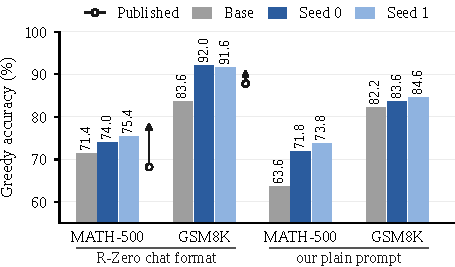
\includegraphics[width=\columnwidth]{figures/figA_rzacc.pdf}
\caption{Greedy accuracy (\%) of R-Zero's final solvers (iteration 3) and the base model. Arrows: the published base and final accuracy \citep{huang2026rzero}, which use GPT-4o as answer judge. Our GSM8K set is 500 test problems.}
\label{fig:rzacc}
\end{figure}

\begin{figure}[htbp]
\centering
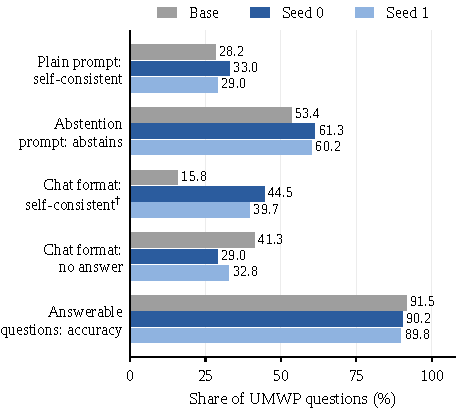
\includegraphics[width=\columnwidth]{figures/figA_rzero.pdf}
\caption{R-Zero's final solvers on UMWP. Under the plain prompt, the paired 95\% CIs of the rise in self-consistent answers are $[1.3, 8.3]$ (seed 0) and $[-2.5, 4.0]$ (seed 1)$^{\dagger}$, from 10,000 item-bootstrap resamples.}
\label{fig:rzero}
\end{figure}

\FloatBarrier
\section{Further Results}
\label{app:results}

Figure~\ref{fig:perseed} shows the ill-posed share of every labelled round, and Figure~\ref{fig:sizes} the size of every training set. \emph{Post-trained scorers.} Post-trained models act as sharpened solvers: the band admits 75\% and 76\% ill-posed problems from the fixed pool when Qwen3-14B and Qwen2.5-32B-Instruct score it, against 64\% and 62\% for their base models (pre-registered). \emph{Reward variants.} Offering \unk{} without reward lowers abstention on unanswerable UMWP questions to 31--38\% (full curriculum: 69--71\%; base model: 53\%) and raises the frontier of \S\ref{sec:remedies} to 23\%. Letting \unk{} win the vote raises abstention on premise-deleted problems by 8--13 points and, in a continued loop, cuts the ill-posed problems trained toward an invented answer to 49--61\% in round four (full curriculum: 79--81\%), rising back to 63--75\% in round five; one of three seeds then abstains on 95\% of intact problems. With a triple weight, the share of training samples answering \unk{} reaches 100\% within 22 and 40 steps, and one seed's accuracy falls from 82\% to 21\%.

\begin{figure}[htbp]
\centering
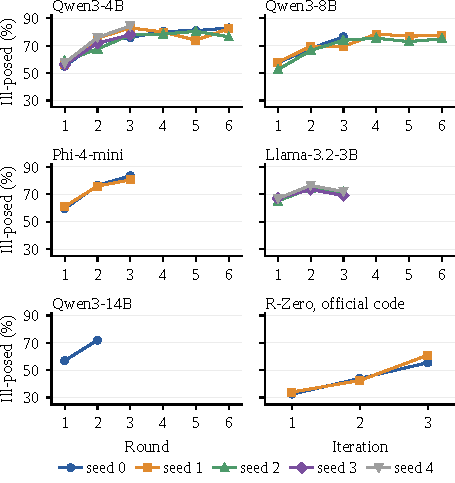
\includegraphics[width=\columnwidth]{figures/figA_perseed.pdf}
\caption{Ill-posed share (\%) of the admitted curriculum per lineage (200 labelled problems per seed and round or iteration). Llama seeds 0 and 1 collapsed in round 1 and seed 2 after round 3 (accuracy below half the base model's, or most MATH samples truncated).}
\label{fig:perseed}
\end{figure}

\begin{figure}[htbp]
\centering
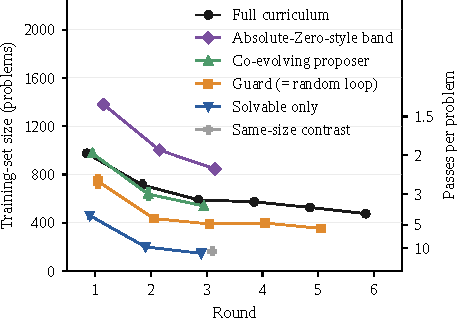
\includegraphics[width=\columnwidth]{figures/figA_sizes.pdf}
\caption{Training-set size of the Qwen3-4B curricula by round (bars: range over seeds; right axis: passes per problem, $1{,}920/n$). Seeds: full curriculum 0--4 (0--2 from round 4), Absolute-Zero-style band 0--1, co-evolving proposer 0--3, abstention guard 0--2, solvable only 0--3, same-size contrast 0--4 (both arms). The size-matched random loop matches the guard's size in every seed and round. Training sets include the admitted planted problems.}
\label{fig:sizes}
\end{figure}

\begin{table}[tbp]
\centering
\small
\begin{tabular}{p{0.93\columnwidth}}
\toprule
\emph{Inconsistency (contradictory condition).} ``[\dots] The pizza is cut into 8 equal slices. Emily and her 3 siblings each eat 2 slices, but 1 slice goes uneaten. If their friend Joe eats all the uneaten slices, how many more slices than Emily did he eat?'' \\
\addlinespace
\emph{Underspecification (missing premise).} ``[\dots] a square-shaped venue measures 100 feet on each side. If the venue charges \$15 for each ticket and sells 70\% of its total seating capacity, how much money does the venue earn from ticket sales?'' \\
\addlinespace
\emph{Ambiguity (ambiguous reference).} ``[\dots] 25 dimes in her piggy bank. She found 15 more dimes that afternoon, exchanged them for quarters, and then divided the quarters equally among her 5 grandchildren. How many cents did each grandchild receive?'' (\emph{them}: 15 or 40 dimes?) \\
\bottomrule
\end{tabular}
\caption{Problems admitted in round 3 of the Qwen3-4B loop; the kind follows the judges' notes. In a blind typing of 540 labelled ill-posed problems, contradictory or impossible conditions lead at every round (38--43\%), ahead of missing premises (18--29\%) and ambiguous references (14--17\%).}
\label{tab:examples}
\end{table}

\paragraph{Closed loops and offline rules.} The rules of Table~\ref{tab:filters} were applied offline; its classifier is a 5-fold cross-validated logistic regression on agreement under both prompts, abstention share, agreement between the prompts' answers, length and number count. As closed loops on Qwen3-4B we ran the band, the abstention guard and the size-matched random loop (seeds 0--2), the co-evolving proposer (seeds 0--3), Absolute Zero's rule (seeds 0 and 1) and a recalibrated band (seeds 0 and 1, and Llama-3.2-3B seed 1; three rounds). In each round, the recalibrated band chooses the agreement limits on the grid $k/8$, with the upper limit at most $7/8$, that maximise the admission rate of the planted intact problems minus that of their deleted twins, admitting at least 30\% of the intact ones; it uses no answer labels, but the planted problems are of known status. Its admitted proposals are 29.5\% and 37.0\% unsolvable at round one and 50.5\% and 35.0\% at round three, against 64.5\% and 66.5\% under the fixed band, and the in-band rate of deleted relative to intact planted problems rises from 0.59 and 0.46 to 1.25 and 1.16 (Llama: 0.68 to 1.00, with 31.0\% to 55.0\% unsolvable). The recalibration delays and lowers the drift, but by round three the band again admits deleted problems more readily than intact ones.

\paragraph{Cross-seed consensus$^{\dagger}$.} On the 205 UMWP questions that all three round-5 seeds answer self-consistently (answers read as in \S\ref{sec:setting}), the seeds give the same answer on 181 (88.3\%, Wilson 95\% interval 83.2--92.0). On 141 of these (77.9\%) the common answer is the base model's most frequent answer, and on 155 (85.6\%) it is one of its most frequent answers when these are tied; on 170 (93.9\%) it is among the base model's eight answers, and over all 181 the base model gives it in 3.7 of eight samples on average. The match is 96 of 100 (96.0\%) where the base model was itself self-consistent and 45 of 81 (55.6\%) where it was not. Each seed's modal answer equals the base model's on 73--76\% of the 205 questions, and the common answer equals the answer of the answerable original on 54.7\%. On the 112 readings questions (fresh samples), all three seeds answer 31 self-consistently, agree on 23, and give the base model's most frequent answer on 18 of these (78.3\%; 20, or 87.0\%, counting ties). Probe samples that share a sampling index agree with the base model's samples at most slightly more often than samples with different indices (0.30--0.31 against 0.26--0.30).

\begin{figure}[htbp]
\centering
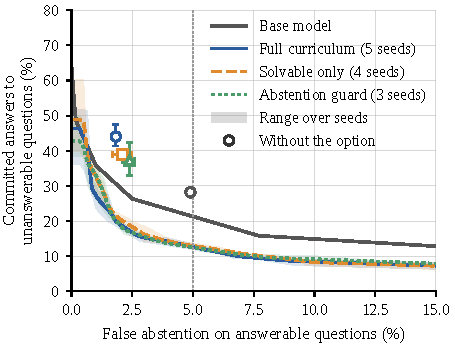
\includegraphics[width=\columnwidth]{figures/fig4_frontier.pdf}
\caption{Selective answering on UMWP with the abstention option (Qwen3-4B, round 3). Each line is the frontier of label-free rules that answer only when enough of the eight samples agree or few of them abstain, averaged over seeds (shaded: range over seeds). Hollow markers: self-consistent answers under the plain prompt, placed at the model's false-abstention rate with the option (mean over seeds; bars: range). Dotted line: the 5\% rate used in \S\ref{sec:remedies}. Calibrated on a random half of the question pairs (stratified by source; both directions averaged)$^{\dagger}$, the rules reach 16.3--18.9\% at the guard's false-abstention rate (achieved 2.2--3.4\%) and 12.4--13.1\% at 5\% (achieved 4.4--5.6\%), against 16.8--17.8\% and 12.1--13.5\% in sample; the base model reaches 20.7\% (21.3\% in sample). Over 200 random splits, the means are 16.9--18.0\% and 12.2--13.0\%. Under the plain prompt, the guard-trained solver answers 33--42\% of the unanswerable questions self-consistently. Answers are read as in \S\ref{sec:setting}; the frontiers change by at most 0.2 points from the first parser's.}
\label{fig:frontier}
\end{figure}

\FloatBarrier
\section{Readings Annotation}
\label{app:readings}

We selected 112 unanswerable UMWP questions and 112 answerable ones that the base model solves in at most three of eight samples, matched on base agreement (40, 69 and 3 questions at agreement 2, 3 and 4 of 8). The base model and the round-5 solvers of three seeds each produced eight fresh solutions per question (896 units of eight solutions). LLM labellers (Claude Opus, one fresh context per batch; they saw the question and the last 1,800 characters of each solution, but not the model, round, seed or answerability) grouped the solutions of each unit into readings of the text, flagged each solution that notes missing, ambiguous or contradictory information or states an assumption it had to make, and labelled the source of disagreement (different readings, computation errors, both, or none). A second pass by fresh labellers on a random quarter of the base units agrees at $\kappa{=}0.91$ on the source of disagreement and $\kappa{=}0.93$ on the flags, and matches the number of readings exactly in 86\% of units.

\paragraph{By category$^{\dagger}$.} From base to round five (pooled over seeds), the number of readings per question and the share of flagged samples change as follows: missing key information (36 questions), 4.17 to 2.84 and 12.8\% to 60.3\%; ambiguous key information (58), 3.98 to 2.92 and 19.2\% to 69.0\%; unrealistic conditions (10), 2.80 to 2.97 and 7.5\% to 38.8\%; unrelated object (6), 2.83 to 2.22 and 4.2\% to 31.2\%; missing question (2), 3.50 to 4.00 and 1 of 16 to 6 of 48 samples.

\paragraph{Stricter thresholds$^{\dagger}$.} Figure~\ref{fig:thresholds} shows the share of unanswerable UMWP questions answered self-consistently at stricter thresholds. The rise holds at every threshold and is proportionally larger at the stricter ones; ties at the top concern at most 2.2\% of questions.

\begin{figure}[htbp]
\centering
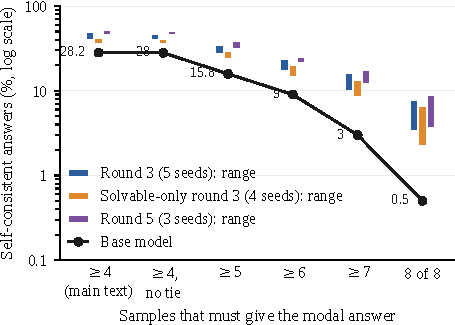
\includegraphics[width=\columnwidth]{figures/figA_thresholds.pdf}
\caption{Self-consistent answers (\%, log scale) to the 600 unanswerable UMWP questions under the plain prompt, by the number of the eight samples that must give the most frequent numeric answer (Qwen3-4B; bars: range over seeds).}
\label{fig:thresholds}
\end{figure}

\paragraph{Exact match.} The labellers' label for no disagreement (``all final answers equal'') is lenient: it covers 13--37\% of the unanswerable questions after five rounds, whereas all eight answers coincide on 1.8--4.5\%$^{\dagger}$ (none at base under either count); in the 69 further units it covers, the most frequent numeric answer holds zero to seven of the eight samples (median two), and in 50 of them at least five samples decline: the samples agree on declining. Section~\ref{sec:readings} reports the exact count.

\paragraph{Human check (pre-registered).} Two external annotators labelled, independently, without AI assistance and blind to model, round and the LLM labels, in two differently ordered versions, the 184 base units not used in a first packet (92 unanswerable, 92 hard answerable; source of disagreement) and 600 single solutions (two base and two round-5 solutions for each of the 112 unanswerable and 38 answerable questions; flag and answer status). They label 88.0\% of the unanswerable units as disagreeing over readings, against 16.3\% of the hard answerable ones (difference $+0.72$, 95\% CI $[0.63, 0.80]$; LLM labels on the same units: $+0.67$), and their flag rate on unanswerable questions rises from 14.3\% at base to 58.0\% at round five ($+0.44$, CI $[0.36, 0.51]$; LLM: $+0.43$): both pre-registered criteria are met. Agreement with the LLM labels is $\kappa{=}0.84$ and $0.76$ for the two annotators on readings (binary), $0.72$ and $0.59$ on the four-way source and $0.96$ and $0.91$ on flags; between the annotators it is $0.80$, $0.69$ and $0.94$. The annotators also judge that 29.7\% of the round-5 solutions to unanswerable questions give no final numeric answer, mostly because they decline in words (``cannot be determined'', ``Answer: N/A''), against 2.2\% under the parser our probes first used, which then read the last number of the text$^{\dagger}$. The strict reading of \S\ref{sec:setting}, which treats such declines, answers in a variable and solutions without a final number as non-answers, ignores text after a new question that the model writes itself, and otherwise takes the same number, agrees with the annotators on 94.6\% of the solutions (first parser: 85.5\%): it reads 5\% of the solutions they call numeric answers as non-answers and misses 10\% of their non-answers (first parser: 2\% and 92\%), so it errs, if anything, toward fewer self-consistent answers. A first packet for this check was replaced by these new items before any of its labels was analysed (Appendix~\ref{app:prereg}, deviation 15).

\paragraph{Re-measurement with saved texts$^{\dagger}$.} The first UMWP probes kept only the parsed answers. We therefore re-ran the same probes (prompt, sampling and seed) with texts saved on every checkpoint behind a UMWP or external-set number in the paper, 89 runs in all, and read each run with both parsers; the plan and the read scripts were logged before any new output was read, the main read script reproduces the earlier numbers exactly on the original runs, and two corrections were logged before the main read was run: the strict reading keeps the first parser's number wherever it finds one, and it cuts a solution at a new question the model writes itself, which base models often do (Qwen3-8B-Base in 53\% of its samples); the second came after an interim look at completed runs, in which the uncut reading lowered Qwen3-8B-Base's accuracy on the answerable originals from 74\% to 50\%. Under the first parser the new runs reproduce the old ones (base 28.5\% against 28.7\%; round three 57--75\% against 59--76\%), so the differences come from the parser, not from sampling, which is not bitwise reproducible on GPUs. Under the strict reading, the base model declines in words in 3\% of its samples on unanswerable questions and the round-3 solvers in 13--22\%, and the self-consistent-answer rate is 28\% at base, 41--48\% at round three and 48--50\% at round five; Qwen3-8B-Base, whose solutions the first parser often read from a question it had written itself, rises from 26\% instead of 7\%. All UMWP and external-set numbers in the paper come from these runs under the strict reading; registered outcomes keep the parser they were scored with (Appendix~\ref{app:prereg}, deviation 16). On the 112 questions of Figure~\ref{fig:accommodation}, the strict reading changes the rate from 12.5\% to 14.3\% at base, from 61--75\% to 40--46\% at round three and from 63--79\% to 41--49\% at round five. Re-run so that generation itself stops at a new question, as in the loop's filter$^{\dagger}$, seven checkpoints give 30.0\% for Qwen3-4B-Base (cut reading: 28.2\%), 40.8\% and 43.7\% for two of its round-3 solvers (41.3\% and 43.3\%), and 28.2\% and 36--41\% for Qwen3-8B-Base and its round-3 solvers (26.0\% and 34--38\%): cutting slightly understates the base models, whose cut solutions sometimes ran on to the length limit, and the rise stays. One known flaw of the frozen reading: its decline pattern for ``N/A'' also matches words ending in ``na'', such as the name Tina, in solutions without an ``Answer:'' line; restricting it to a stand-alone N/A changes the self-consistent-answer rates by at most 0.2 points for Qwen3-4B and Phi-4-mini and by 0.5--0.7 points for Qwen3-8B$^{\dagger}$. The analyses of band membership (\S\S\ref{sec:drift}--\ref{sec:mechanism}) read answers as the loop's filter does, which stops at a new question and takes a verbal decline's last number, as the first parser does; under the strict reading their conclusions hold, but about half of the unanswerable questions that leave the band do so by declining. The secondary premise-deleted probe keeps the first parser.

\FloatBarrier
\section{Further Related Work}
\label{app:related}

\paragraph{Label-free self-play and rewards.} R-Zero, Absolute Zero, SeRL and self-questioning models admit problems by the solver's agreement or learnability \citep{huang2026rzero,zhao2025absolute,fang2025serl,chen2025sqlm}, TTRL rewards the majority answer \citep{zuo2025ttrl}, grounded variants add labels or teachers \citep{yu2025rfew,sundaram2026soar}, and self-play extends to other tasks \citep{yang2026spell,huang2026gzero,yu2026chase,cowsik2026selfplay}, whose players can game their rewards \citep{bailey2026sgs,zhou2026convincing}. Vocabulary Dropout notes that disagreement cannot tell hard from ill-posed problems \citep{dineen2026vocabulary}; for a fixed post-trained model, D\'ej\`aQ finds high-learnability problem--answer pairs more often incorrect \citep{ropke2026dejaq}; OpenSIR, that lowering its solve-rate threshold lowers validity, measured as agreement of GPT-5's majority answer with the reference, while validity judged by humans rises during training at its default threshold \citep{kwan2025opensir}; and data gating decides whether code self-play stays stable \citep{pu2026survive}. Beyond these, we audit admitted sets over rounds, locate the drift in differential exit on a fixed pool, separate challenger from selection in the official R-Zero code and trace the effect on the solver's answers; we ask whether a problem's text determines a unique answer, not whether a proposed answer is correct. Other label-free objectives reward self-consistency, confidence or low entropy \citep{huang2023lmsi,prasad2025scpo,zhao2026intuitor,prabhudesai2025rent,zhang2025empo,agarwal2025entropy}, sharpening a model toward its initial mode even when wrong \citep{huang2025sharpening,he2026howfar,shafayat2025srt}; with labels, DAPO drops groups the solver always or never solves \citep{yu2025dapo}, and spurious rewards raise Qwen accuracy \citep{shao2026spurious}.

\paragraph{Uncertainty-based selection.} Sampling disagreement \citep{wang2023selfconsistency,kuhn2023semantic,farquhar2024semantic} mixes epistemic uncertainty, which training reduces, with aleatoric uncertainty, which it cannot \citep{kendall2017uncertainties,hullermeier2021aleatoric}. Selection by uncertainty or loss is drawn to noisy, unlearnable points \citep{karamcheti2021outliers,mindermann2022rholoss}, hence BALD's epistemic score \citep{houlsby2011bald}, as curiosity is drawn to a noisy TV \citep{burda2019curiosity}; training dynamics separate ambiguous from hard examples \citep{swayamdipta2020cartography}, and curricula target the frontier of learnability \citep{bengio2009curriculum,jiang2021plr,dennis2020paired}. Self-play compounds this pull round after round.

\paragraph{Abstention, presupposition and ambiguity.} QA has long studied unanswerable questions \citep{rajpurkar2018squad2,kamath2020selective}; language models partly know what they do not know \citep{kadavath2022know,yin2023selfaware} and can be tuned to say so \citep{zhang2024rtuning,wen2025abstention}. Reinforcement fine-tuning reduces refusal on unanswerable math \citep{song2025hallucination}, reasoning models flag uncertainty yet still answer \citep{kirichenko2025abstentionbench,gu2026detection}, and abstention rewards can collapse into refusal \citep{che2026abstention}; these works start from labelled answerability \citep{tong2026aca}, whereas the behaviour we study comes from a label-free curriculum. NLP has also studied questions with false or questionable presuppositions \citep{karttunen1974presupposition,kim2021linguist,kim2023qa2,yu2023crepe,hu2023falsepremise} and ambiguous or underspecified ones \citep{min2020ambigqa,liu2023ambient,cole2023selectively,hou2024decomposing,li2025questbench}.
